\documentclass[14pt]{extbook}
\usepackage{multicol, enumerate, enumitem, hyperref, color, soul, setspace, parskip, fancyhdr} %General Packages
\usepackage{amssymb, amsthm, amsmath, bbm, latexsym, units, mathtools} %Math Packages
\everymath{\displaystyle} %All math in Display Style
% Packages with additional options
\usepackage[headsep=0.5cm,headheight=12pt, left=1 in,right= 1 in,top= 1 in,bottom= 1 in]{geometry}
\usepackage[usenames,dvipsnames]{xcolor}
\usepackage{dashrule}  % Package to use the command below to create lines between items
\newcommand{\litem}[1]{\item#1\hspace*{-1cm}\rule{\textwidth}{0.4pt}}
\pagestyle{fancy}
\lhead{Progress Quiz 1}
\chead{}
\rhead{Version B}
\lfoot{3735-1698}
\cfoot{}
\rfoot{Spring 2021}
\begin{document}

\begin{enumerate}
\litem{
Write the equation of the line in the graph below in Standard form $Ax+By=C$. Then, choose the intervals that contain $A, B, \text{ and } C$.
\begin{center}
    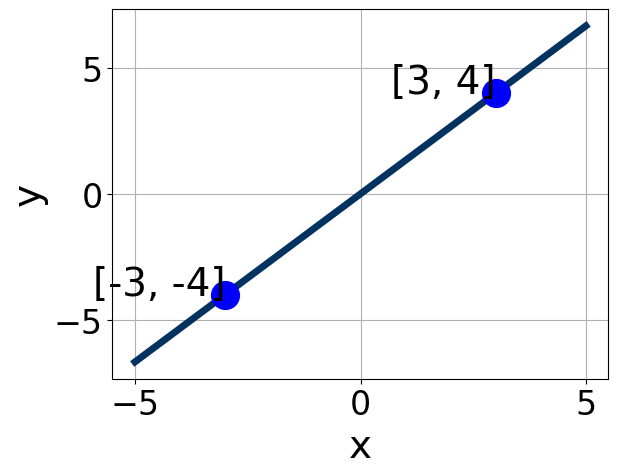
\includegraphics[width=0.5\textwidth]{../Figures/linearGraphToStandardB.png}
\end{center}
\begin{enumerate}[label=\Alph*.]
\item \( A \in [-1.8, 2.2], \hspace{3mm} B \in [-0.2, 2.7], \text{ and } \hspace{3mm} C \in [-3, -2] \)
\item \( A \in [3, 13], \hspace{3mm} B \in [2.6, 5.3], \text{ and } \hspace{3mm} C \in [-16, -12] \)
\item \( A \in [-4, -1], \hspace{3mm} B \in [2.6, 5.3], \text{ and } \hspace{3mm} C \in [-16, -12] \)
\item \( A \in [-1.8, 2.2], \hspace{3mm} B \in [-1.1, -0.1], \text{ and } \hspace{3mm} C \in [1, 4] \)
\item \( A \in [3, 13], \hspace{3mm} B \in [-8.7, -2], \text{ and } \hspace{3mm} C \in [9, 17] \)

\end{enumerate} }
\litem{
Write the equation of the line in the graph below in Standard form $Ax+By=C$. Then, choose the intervals that contain $A, B, \text{ and } C$.
\begin{center}
    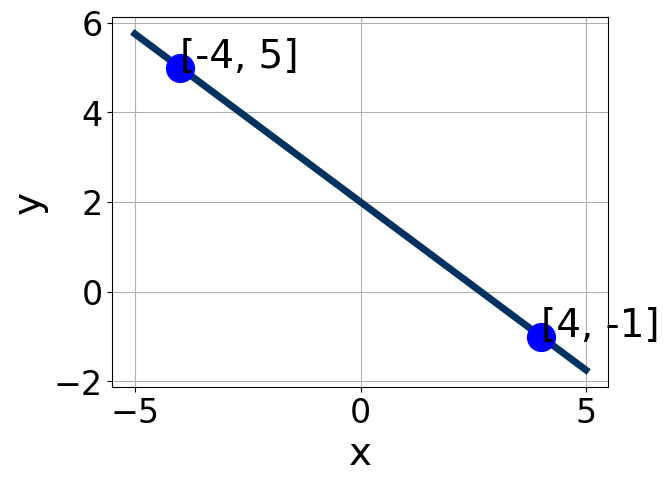
\includegraphics[width=0.5\textwidth]{../Figures/linearGraphToStandardCopyB.png}
\end{center}
\begin{enumerate}[label=\Alph*.]
\item \( A \in [-7.9, -4.6], \hspace{3mm} B \in [2.45, 3.93], \text{ and } \hspace{3mm} C \in [-3.54, -2.43] \)
\item \( A \in [4.8, 5.8], \hspace{3mm} B \in [2.45, 3.93], \text{ and } \hspace{3mm} C \in [-3.54, -2.43] \)
\item \( A \in [-4, -0.8], \hspace{3mm} B \in [-1.83, 0.68], \text{ and } \hspace{3mm} C \in [0.46, 1.89] \)
\item \( A \in [4.8, 5.8], \hspace{3mm} B \in [-3.03, -1.89], \text{ and } \hspace{3mm} C \in [2.5, 3.87] \)
\item \( A \in [-4, -0.8], \hspace{3mm} B \in [0.88, 1.98], \text{ and } \hspace{3mm} C \in [-1.9, 0.29] \)

\end{enumerate} }
\litem{
Find the equation of the line described below. Write the linear equation as $ y=mx+b $ and choose the intervals that contain $m$ and $b$.\[ \text{Perpendicular to } 7 x + 8 y = 11 \text{ and passing through the point } (-4, 6). \]\begin{enumerate}[label=\Alph*.]
\item \( m \in [1.12, 1.35] \hspace*{3mm} b \in [-11.04, -10.43] \)
\item \( m \in [1.12, 1.35] \hspace*{3mm} b \in [9.9, 10.48] \)
\item \( m \in [0.51, 1.09] \hspace*{3mm} b \in [10.26, 11.23] \)
\item \( m \in [1.12, 1.35] \hspace*{3mm} b \in [10.26, 11.23] \)
\item \( m \in [-1.3, -1.04] \hspace*{3mm} b \in [-0.01, 2.22] \)

\end{enumerate} }
\litem{
First, find the equation of the line containing the two points below. Then, write the equation as $ y=mx+b $ and choose the intervals that contain $m$ and $b$.\[ (-8, 9) \text{ and } (-3, -4) \]\begin{enumerate}[label=\Alph*.]
\item \( m \in [-3.6, -0.6] \hspace*{3mm} b \in [9.8, 16.8] \)
\item \( m \in [-3.6, -0.6] \hspace*{3mm} b \in [-8, 0] \)
\item \( m \in [-2.4, 3.6] \hspace*{3mm} b \in [2.8, 6.8] \)
\item \( m \in [-3.6, -0.6] \hspace*{3mm} b \in [16, 20] \)
\item \( m \in [-3.6, -0.6] \hspace*{3mm} b \in [-11.8, -10.8] \)

\end{enumerate} }
\litem{
Solve the equation below. Then, choose the interval that contains the solution.\[ -8(18x + 3) = -9(-10x + 2) \]\begin{enumerate}[label=\Alph*.]
\item \( x \in [-0.31, -0.15] \)
\item \( x \in [-0.07, -0.02] \)
\item \( x \in [0.06, 0.23] \)
\item \( x \in [-0.86, -0.73] \)
\item \( \text{There are no real solutions.} \)

\end{enumerate} }
\litem{
Find the equation of the line described below. Write the linear equation as $ y=mx+b $ and choose the intervals that contain $m$ and $b$.\[ \text{Parallel to } 3 x - 4 y = 5 \text{ and passing through the point } (-7, -10). \]\begin{enumerate}[label=\Alph*.]
\item \( m \in [0.4, 1.32] \hspace*{3mm} b \in [2.8, 6] \)
\item \( m \in [1.04, 1.99] \hspace*{3mm} b \in [-6, -4.1] \)
\item \( m \in [0.4, 1.32] \hspace*{3mm} b \in [-3.2, -1.3] \)
\item \( m \in [0.4, 1.32] \hspace*{3mm} b \in [-6, -4.1] \)
\item \( m \in [-0.92, -0.49] \hspace*{3mm} b \in [-15.4, -15] \)

\end{enumerate} }
\litem{
Solve the equation below. Then, choose the interval that contains the solution.\[ -9(5x -4) = -16(-15x -3) \]\begin{enumerate}[label=\Alph*.]
\item \( x \in [-0.3, -0.1] \)
\item \( x \in [-0.67, -0.31] \)
\item \( x \in [0.12, 0.41] \)
\item \( x \in [-0.17, 0.04] \)
\item \( \text{There are no real solutions.} \)

\end{enumerate} }
\litem{
Solve the linear equation below. Then, choose the interval that contains the solution.\[ \frac{-7x + 4}{3} - \frac{-7x -9}{4} = \frac{4x + 5}{5} \]\begin{enumerate}[label=\Alph*.]
\item \( x \in [5.18, 6.98] \)
\item \( x \in [-1.7, -0.92] \)
\item \( x \in [1.74, 2.35] \)
\item \( x \in [0.45, 1.14] \)
\item \( \text{There are no real solutions.} \)

\end{enumerate} }
\litem{
First, find the equation of the line containing the two points below. Then, write the equation as $ y=mx+b $ and choose the intervals that contain $m$ and $b$.\[ (10, -9) \text{ and } (-9, -2) \]\begin{enumerate}[label=\Alph*.]
\item \( m \in [-1.12, 0] \hspace*{3mm} b \in [-19.4, -16.8] \)
\item \( m \in [-1.12, 0] \hspace*{3mm} b \in [5.7, 7.1] \)
\item \( m \in [-1.12, 0] \hspace*{3mm} b \in [-7, -3.3] \)
\item \( m \in [-1.12, 0] \hspace*{3mm} b \in [3.9, 6.3] \)
\item \( m \in [0.33, 0.65] \hspace*{3mm} b \in [0.1, 2.4] \)

\end{enumerate} }
\litem{
Solve the linear equation below. Then, choose the interval that contains the solution.\[ \frac{8x -8}{7} - \frac{-5x -7}{5} = \frac{4x + 5}{2} \]\begin{enumerate}[label=\Alph*.]
\item \( x \in [15.7, 17.7] \)
\item \( x \in [40, 45] \)
\item \( x \in [-2.75, 1.25] \)
\item \( x \in [32.3, 38.3] \)
\item \( \text{There are no real solutions.} \)

\end{enumerate} }
\end{enumerate}

\end{document}